\documentclass[11pt]{article}

\usepackage[margin=2.5cm]{geometry}
\usepackage[T1]{fontenc}
\usepackage{amsmath,amssymb,amsthm}
\usepackage{booktabs}
\usepackage{longtable}
\usepackage{array}
\usepackage[shortlabels]{enumitem}
\usepackage{xcolor}
\usepackage{tikz}
\usetikzlibrary{arrows.meta,positioning}
\usepackage{caption}
\usepackage{subcaption}
\usepackage{parskip}
\usepackage{hyperref}

% ---------------------------------------------------------------------------
% Colors (loosely matching the companion web artifact's palette)
% ---------------------------------------------------------------------------
\definecolor{accentc}{HTML}{2A4FC7}   % set to the counterfactual value
\definecolor{respondc}{HTML}{B8730E}  % responds / recomputed
\definecolor{naturalc}{HTML}{6B7280}  % kept at natural / recorded value
\definecolor{reusec}{HTML}{1E8F82}    % REUSE tag
\definecolor{newc}{HTML}{B23A63}      % NEW tag
\definecolor{feasyesc}{HTML}{2F7D3F}
\definecolor{feasmodc}{HTML}{B8860B}
\definecolor{feasnoc}{HTML}{B33A3A}

\hypersetup{
  colorlinks=true,
  linkcolor=accentc,
  citecolor=accentc,
  urlcolor=accentc,
  pdftitle={Causal Dependence Plots --- Project Notes},
  pdfauthor={RAI}
}

% ---------------------------------------------------------------------------
% Convenience macros (mirror the Markdown vault's REUSE/NEW/open-question style)
% ---------------------------------------------------------------------------
\newcommand{\reusetag}[1]{\textcolor{reusec}{\textbf{[REUSE: #1]}}}
\newcommand{\newtag}{\textcolor{newc}{\textbf{[NEW]}}}
\newcommand{\feasyes}{\textcolor{feasyesc}{$\bullet$}~intern-feasible}
\newcommand{\feasmod}{\textcolor{feasmodc}{$\bullet$}~moderate supervision}
\newcommand{\feasno}{\textcolor{feasnoc}{$\bullet$}~supervisor-owned}

\newenvironment{openquestions}{%
  \par\smallskip\noindent\textbf{Open questions}%
  \begin{itemize}[leftmargin=1.4em]
}{%
  \end{itemize}\par
}

% ---------------------------------------------------------------------------
% TikZ styles shared by every ECM/intervention diagram (see sec. Big picture)
% ---------------------------------------------------------------------------
\tikzset{
  defaultnode/.style={rectangle, rounded corners=2pt, draw=black!55, fill=white,
    minimum width=1.6cm, minimum height=0.85cm, font=\small, align=center},
  accentnode/.style={defaultnode, draw=accentc, fill=accentc, text=white},
  respondnode/.style={defaultnode, draw=respondc, fill=respondc, text=white},
  naturalnode/.style={defaultnode, draw=naturalc, fill=naturalc!15, text=naturalc},
  targetnode/.style={defaultnode, draw=black, line width=1.1pt},
  normaledge/.style={-{Stealth[length=2.4mm]}, draw=black!70, line width=0.75pt},
  severededge/.style={-{Stealth[length=2.4mm]}, draw=black!45,
    dash pattern=on 3pt off 2pt, line width=0.75pt},
  accentedge/.style={-{Stealth[length=2.4mm]}, draw=accentc, line width=1.2pt},
}

\title{Causal Dependence Plots\\[4pt]\large Project Notes --- RAI}
\author{}
\date{\today}

\begin{document}
\maketitle
\tableofcontents

\section*{How to use these notes}
\label{sec:howto}
\addcontentsline{toc}{section}{How to use these notes}

This document is the working knowledge base for the project, kept separate
from \texttt{docs/} (the mentor's source material, which stays unedited so
it is always safe to check a note against what was actually handed to us).

\subsection*{Layout}

\begin{description}[leftmargin=2.2em]
  \item[\texttt{main.tex}] the master file: preamble, macros, TikZ styles,
    and the \verb|\input| list below.
  \item[\texttt{sections/}] one file per topic, mirroring the handout's own
    structure (\texttt{docs/CDP\_explainer\_students.pdf}). Compile order
    equals reading order.
  \item[\texttt{recall.tex}] a \emph{separate}, standalone self-quiz document
    (compiles to its own \texttt{recall.pdf}) --- questions first, answers
    at the end, for testing yourself \emph{without} this reference open.
    Add to it as you read further; don't fold it into \texttt{main.tex}.
\end{description}

Build with \texttt{latexmk -pdf main.tex} (or \texttt{pdflatex} run twice, so
the table of contents and cross-references settle).

\subsection*{Conventions}

\begin{itemize}
  \item \textbf{Cross-references}: every section carries a
    \verb|\label{sec:...}|; refer to it elsewhere with \verb|\ref| or
    \verb|\hyperref[sec:...]{...}| rather than repeating content.
  \item \textbf{REUSE vs.\ NEW}: the mentor's handout tags every idea as
    applying an existing result or contributing a new one. Kept here as the
    \verb|\reusetag{Source}| / \verb|\newtag| macros (defined in
    \texttt{main.tex}), rendering as \reusetag{Source} / \newtag. This tag is
    the organizing device for the whole project --- keep using it.
  \item \textbf{Cite by section}: when a note is based on the handout,
    reference its section number (e.g.\ ``handout \S1.3'') so it is easy to
    jump back to the PDF and check nuance.
  \item \textbf{Don't edit \texttt{docs/}}: if a note turns out to be wrong
    once something is understood better, fix the note, not the memory of the
    PDF --- the PDF is the ground truth handed down from the mentor.
\end{itemize}

\subsection*{Day to day}

\begin{enumerate}
  \item When a source is read (paper, handout section), add a dated entry to
    the reading log (\S\ref{sec:reading-log}) --- even two lines.
  \item Pull any new term into the glossary (\S\ref{sec:glossary})
    immediately, before the exact definition used \emph{in this project} is
    forgotten (causal-inference terms often carry paper-specific
    conventions).
  \item When a section grows past its own topic, split it into a new file
    under \texttt{sections/} and add an \verb|\input| line in
    \texttt{main.tex} --- but don't pre-create empty sections for material
    not yet read.
  \item Anything unresolved goes to the open-questions section
    (\S\ref{sec:questions}) instead of sitting half-understood inside a
    content section.
\end{enumerate}

\subsection*{Starting scaffold}

The content sections were seeded from \texttt{docs/CDP\_explainer\_students.pdf}
(\S0--\S2) and the CDP paper's introduction (arXiv:2303.04209, \S1 $+$ start
of \S2.1). They are \textbf{not exhaustive} --- most of the arXiv paper's
\S2 (\S2.1--2.6, its own careful methodology section, per the mentor's
prescribed reading order) has not been folded in yet, nor has the Loftus
``Trustworthy Causal Explanations'' slides (now read, see the reading log)
or a full pass of the IML PDP chapter. Treat the seeded notes as a skeleton
to correct and extend while actually reading, not as a finished summary.

\textbf{Mentor's prescribed reading order} (given 2026-09-19, see the
reading log): (1) Molnar's PDP chapter; (2) the CDP paper,
arXiv:2303.04209, \S1--2 carefully, skim the rest; (3) this project
explainer, \texttt{docs/CDP\_explainer\_students.pdf}. Follow that order,
not whatever order these notes happen to be organized in.

\section{Assumed background}
\label{sec:background}

\emph{Source: handout preamble (``Assumed background: DAGs, the do-operator,
backdoor adjustment, potential outcomes, regression, a little machine
learning.'').} Everything from \S\ref{sec:bigpicture} onward leans on all six
of these.

\textbf{Running example}, used throughout: age $W \to$ exercise $A \to$
weight $M \to$ blood pressure $R$; a model $f$ predicts 10-year
cardiovascular risk, $\hat Y = f(X)$.

\subsection{Notation}
\label{sec:notation}

A quick-reference table for every symbol used in these notes --- consult it
whenever a formula reads ``obviously'' but isn't.

\begin{longtable}{@{}p{3.0cm}p{10.2cm}@{}}
\toprule
\textbf{Symbol} & \textbf{Meaning} \\
\midrule
\endhead
$W, A, M, R$ & The running example's features: age, exercise, weight,
  blood pressure (in that causal order). \\
$X$ & The full feature vector, e.g.\ $(W,A,M,R)$; $X_{-A}$ means ``all
  features except $A$.'' \\
$f$ & The fitted prediction model being explained (any learner). \\
$\hat Y$ & The model's output, added to the causal graph as a node,
  $\hat Y = f(X)$. \\
$Y^*$ & The ``constructed outcome'' $f(X)$ treated as a variable for
  causal-inference purposes --- the same quantity as $\hat Y$, written
  differently depending on whether the point being made is graphical
  ($\hat Y$) or statistical ($Y^*$). \\
$P(\cdot)$, $P(dw)$ & A probability distribution; $P(dw)$ is shorthand for
  integrating/summing against the distribution of $W$ (treat it as
  ``weighted by how $W$ is actually distributed in the population''). \\
$E[\cdot]$, $E_W[\cdot]$ & Expectation; a subscript names which variable's
  distribution the average is taken over. \\
$\operatorname{do}(A=a)$ & Pearl's do-operator: \emph{set} $A$ to $a$ by
  intervention (delete the arrow into $A$), as opposed to conditioning on
  $A=a$ in observational data (see below). \\
$\perp$ & Statistical independence, e.g.\ $\{R(a)\}\perp A \mid W$ reads
  ``independent of $A$, once you condition on $W$.'' \\
$\theta(a)$ & The population target of a dependence plot at level $a$
  (e.g.\ the average TDP, Eq.~\ref{eq:tdp-backdoor}). \\
$\hat\theta(a)$ & An \emph{estimator} of $\theta(a)$ from data. A hat over
  any symbol ($\hat\mu$, $\hat\pi$, $\hat{\mathrm{se}}$, \dots) always means
  ``estimated from a finite sample,'' as opposed to the population quantity
  underneath it. \\
$\mu(a,z)$ & The outcome regression, $E[Y^* \mid A=a, Z=z]$
  (\S\ref{sec:estimation}). \\
$\pi(a\mid z)$ & The propensity/treatment regression, $P(A=a\mid Z=z)$
  (\S\ref{sec:estimation}). \\
$Z$ & A generic adjustment/covariate set (e.g.\ the parents $W$, or a
  larger valid set) --- kept as a separate letter from the running
  example's $W,M,R$ so formulas stay general across choices of adjustment
  set. \\
$Q(dr\mid a,w)$ & The \textbf{reduced form}: the conditional law of the
  non-parent features given $(A,W)$ (\S\ref{sec:identification}). \\
$\Psi(a)$ & The \textbf{bridge mean} $E[Y(A,Z(a))]$ that the NIDP turns out
  to equal (\S\ref{sec:identification}). \\
$\sqrt{n}$ (rate) & Shorthand for ``a regular estimator whose error shrinks
  like $1/\sqrt n$'' --- the standard, non-exotic rate that licenses
  ordinary $\hat\theta \pm 1.96\,\hat{\mathrm{se}}$ confidence intervals. \\
$o_p(n^{-1/2})$ & ``Shrinks faster than $1/\sqrt n$, in probability'' ---
  the condition cross-fitting needs the \emph{product} of two nuisance
  errors to satisfy (\S\ref{sec:estimation}). \\
$g_k(a)$, $B_k$, $\psi_k$ & A bin's fixed weight function, the bin itself,
  and the resulting bin target $\psi_k = \int_{B_k}\theta(a)g_k(a)\,da$
  (\S\ref{sec:continuous}). \\
$K_h$, $\theta_h$ & A smoothing kernel at bandwidth $h$, and the resulting
  smoothed curve $\theta_h = K_h * \theta$ (\S\ref{sec:continuous}). \\
$J(a)$ & The interaction remainder in
  $\theta(a)-B = [\mathrm{NDDP}(a)-B]+[\mathrm{NIDP}(a)-B]+J(a)$
  (\S\ref{sec:bigpicture}). \\
Partial-$R^2$ & The fraction of otherwise-unexplained variance an
  unmeasured confounder $U$ would need to explain to matter --- the
  currency of the sensitivity analysis in \S\ref{sec:propagation}. \\
\bottomrule
\caption{Notation used throughout these notes.}
\label{tab:notation}
\end{longtable}

\begin{quote}
\textbf{Watch for this overload:} the handout reuses the letter $R$ for two
different things. In the running example, $R$ is \emph{blood pressure}. But
in \S\ref{sec:identification}'s general identification result, $R$ denotes
``the features other than $A$ and its parents $W$'' --- which in the
running example is actually the \emph{pair} $(M, \text{blood pressure})$
together, not blood pressure alone (weight $M$ is also a non-parent of
$A$). Read $R$ as ``blood pressure'' in running-example prose, and as ``the
generic non-parent remainder'' inside reduced-form formulas --- the handout
doesn't distinguish them notationally, so context has to.
\end{quote}

\subsection{DAGs (directed acyclic graphs)}

Nodes are variables, arrows are \emph{direct} causal effects (relative to
the other variables drawn), and ``acyclic'' means no sequence of arrows
loops back to its start. The \textbf{ECM} (explanatory causal model) in this
project is exactly such a graph over the model's features --- an assumption
brought to the explanation, not something derived from $f$ itself.

Vocabulary this project actually uses:
\begin{itemize}
  \item \textbf{Parents} of $A$: nodes with an arrow directly into $A$
    (here, just $W$).
  \item \textbf{Descendants} of $A$: everything reachable by following
    arrows \emph{out} of $A$ (here, $M$, $R$, $\hat Y$).
  \item \textbf{Non-descendants} of $A$: everything else (here, $W$, plus
    anything upstream of or unrelated to $A$) --- the exact set
    \S\ref{sec:estimation}'s covariate-selection result is about.
  \item \textbf{Backdoor path}: a path between $A$ and the outcome that
    starts with an arrow \emph{into} $A$ (i.e.\ runs through a common
    cause) --- the confounding path adjustment needs to block.
\end{itemize}

One caution worth internalizing early: conditioning on the wrong node can
\emph{create} bias rather than remove it (classically, conditioning on a
\textbf{collider} --- a node two arrowheads point into). This is why ``valid
adjustment set'' is a precise graph-theoretic notion (Pearl's backdoor
criterion, next), not just ``control for everything measured.''

\subsection{The do-operator}

Notation $\operatorname{do}(A=a)$: \emph{set} $A$ to $a$ by intervention, as
opposed to \emph{observing} $A=a$ in data that happened to be collected.
The distinction matters whenever $A$ shares a common cause with the outcome:

\begin{itemize}
  \item $P(R \mid A=a)$ --- among people who happen to exercise at level
    $a$ (contaminated by whatever else predicts exercising at that level,
    e.g.\ age).
  \item $P(R \mid \operatorname{do}(A=a))$ --- if everyone were \emph{forced}
    to exercise at level $a$ (severs whatever normally determines $A$, so no
    contamination).
\end{itemize}

Graphically, $\operatorname{do}(A=a)$ means: delete every arrow \emph{into}
$A$ (its value no longer depends on its natural causes), then let everything
else propagate forward as usual. This is exactly what the TDP diagram in
Figure~\ref{fig:four-plots} (\S\ref{sec:bigpicture}) draws as a severed edge
--- TDP and PCDP are literally this operation applied to the ECM.

\subsection{Backdoor adjustment}

\paragraph{What confounding actually is.} Age has \emph{two separate}
effects here: it affects blood pressure directly (general aging, nothing
to do with exercise), and it also affects how much people exercise (for
whatever reason --- older people might exercise more or less than younger
people). Because age drives \emph{both} exercise and blood pressure, a
naive comparison of blood pressure between high- and low-exercisers picks
up two things tangled together: (1) whatever blood pressure difference
exercise itself actually causes, and (2) a spurious difference that's
really just age showing up twice --- once through its direct effect on
blood pressure, once through its effect on who ends up exercising how
much. That second, spurious piece is \textbf{confounding}: age
\emph{confounds} the naive exercise--blood-pressure comparison.
Graphically, it's exactly a \textbf{backdoor path} (\S1.2 above): the path
exercise $\leftarrow$ age $\to$ blood pressure connects exercise and blood
pressure without exercise having to cause anything, simply because they
share a cause.

\paragraph{Why we bother with the marginal-averaging trick.} We don't want
``the correlation between exercise and blood pressure among whoever
happens to be at each exercise level'' (that's contaminated by age, per
above) --- we want ``what blood pressure would look like if the \emph{same}
population, with the \emph{same} age makeup, were compared at different
exercise levels.'' Forcing every exercise level to be evaluated against the
identical, population-wide age distribution (the $P(W=w)$ in
Eq.~\ref{eq:backdoor} below) is precisely how you strip out age's
contribution and isolate exercise's own effect. This is \emph{why} we do
the adjustment at all, not just how.

The bridge from an interventional question to something estimable from
observational data. \textbf{Backdoor criterion}: a covariate set $W$ is
\emph{valid for adjustment} if (a) it contains no descendant of $A$, and
(b) it blocks every backdoor path from $A$ to the outcome.

\paragraph{What ``valid'' buys you, and what goes wrong without it.}
``Valid'' means exactly this: plug $W$ into the formula below, and you get
the \emph{correct} causal quantity $P(R\mid\operatorname{do}(A=a))$ ---
not just some number, the right one. Each half of the criterion guards
against a specific way of getting a \emph{wrong} number instead:
\begin{itemize}
  \item \textbf{Violating (b)} --- a backdoor path left unblocked --- means
    some confounding is still in the room. If there were a second
    confounder, say socioeconomic status $S$, that also affects both
    exercise and blood pressure, and you adjusted only for age (not $S$),
    the path exercise $\leftarrow S \to$ blood pressure would still be
    open. The ``adjusted'' number would still be contaminated by $S$,
    exactly as in the naive calculation above, just by a different amount.
  \item \textbf{Violating (a)} --- including a descendant of $A$ --- can go
    wrong two ways. If the descendant is something $A$ causes on the way
    to the outcome (a \emph{mediator}, like weight $M$, when what you want
    is the \emph{total} effect), conditioning on it blocks part of the very
    effect you're trying to measure --- you'd end up computing something
    closer to a direct effect than a total one. If the descendant is a
    \textbf{collider} (something caused by both $A$ and something else),
    conditioning on it can manufacture a spurious association that wasn't
    there to begin with.
\end{itemize}
When both (a) and (b) hold, the formula
\begin{equation}
  P(R \mid \operatorname{do}(A=a)) \;=\; \sum_w P(R \mid A=a, W=w)\, P(W=w)
  \label{eq:backdoor}
\end{equation}
is \emph{guaranteed} to equal the true interventional quantity --- that
guarantee is the entire content of ``valid.''

\emph{In words:} to get blood pressure's distribution under a forced
exercise level $a$, go age group by age group ($w$), look at blood pressure
among the people who actually exercised at level $a$ within that age group
($P(R\mid A=a,W=w)$), and then combine those age-group numbers into one
overall number by weighting each age group by how common it actually is in
the population ($P(W=w)$) --- not by how common it is among people who
exercise at level $a$.

The crucial move: average over the \textbf{marginal} distribution of $W$
(the actual population mix), not the distribution of $W$ \emph{among people
at $A=a$} --- that second thing is what a naive $E[R\mid A=a]$ implicitly
does, and it is exactly where confounding sneaks back in.

\paragraph{Worked toy version of the running example.} Say age is 50\% young
/ 50\% old \emph{in the population overall} --- i.e.\ combining the
high-exercise and low-exercise groups together, not within each group
separately. (In real data the age mix \emph{inside} the high-exercise group
could easily be, say, 70\% old / 30\% young if older people tend to
exercise more --- that mismatch between each group's own age mix and the
population's age mix is precisely the confounding the adjustment below is
designed to remove.) And (invented purely to illustrate) blood pressure is
as in Table~\ref{tab:toy-backdoor}.

\begin{table}[h]
\centering
\begin{tabular}{lcc}
\toprule
 & high exercise & low exercise \\
\midrule
young & 110 & 120 \\
old   & 130 & 150 \\
\bottomrule
\end{tabular}
\caption{Toy blood-pressure cell means by age and exercise level.}
\label{tab:toy-backdoor}
\end{table}

Adjusted:
\begin{align*}
  \text{high exercise} &: 0.5(110) + 0.5(130) = 120 \\
  \text{low exercise}  &: 0.5(120) + 0.5(150) = 135
\end{align*}
\emph{In words:} for ``high exercise,'' take the blood pressure of a young
high-exerciser (110) and the blood pressure of an old high-exerciser (130),
and average them \emph{using the population's actual 50/50 age split} ---
not whatever age split happens to show up among the high-exercisers in the
data. Do the same for ``low exercise.'' This gives a clean $-15$ causal contrast, because both numbers are averaged over
the \emph{same} 50/50 age split. A naive $E[BP \mid A{=}\text{high}]$ vs.\
$E[BP \mid A{=}\text{low}]$ would instead average each group over
\emph{its own} age mix (however age happens to correlate with exercise in
the data).

\paragraph{Making the naive number concrete.} Suppose that, because older
people happen to exercise less in this data, the high-exercise group is
actually 80\% young / 20\% old, and the low-exercise group is 20\% young /
80\% old (this is the confounding: each group's own age mix differs from
the population's 50/50). The naive, unadjusted comparison uses \emph{each
group's own} age mix:
\begin{align*}
  \text{naive } E[BP\mid A{=}\text{high}] &= 0.8(110) + 0.2(130) = 114 \\
  \text{naive } E[BP\mid A{=}\text{low}]  &= 0.2(120) + 0.8(150) = 144
\end{align*}
giving a naive contrast of $114-144=-30$ --- \emph{twice as large} as the
true $-15$ causal effect computed above. The extra $-15$ is pure
confounding: high-exercisers look even better than they really are (via
exercise) partly because they also skew younger, and younger people have
lower blood pressure regardless of how much they exercise. Adjustment
(forcing both groups to be evaluated at the same 50/50 age split) removes
exactly that extra piece, leaving only exercise's own effect.

\paragraph{Why parents specifically?} The set of all parents of $A$ always
satisfies the backdoor criterion: any path into $A$ must pass through one of
$A$'s parents immediately before reaching it, so conditioning on all parents
blocks every such path. That is why the handout's core formula
($\theta(a) = E_W[E[Y^* \mid A=a, W]]$, $W = $ parents of $A$; see
\S\ref{sec:bigpicture}) can use \emph{just} the parents --- and why
\S\ref{sec:estimation} can then ask whether a \emph{larger} valid set (all
non-descendants) does better on variance, without needing a different
formula.

One distinction worth keeping crisp: \textbf{valid is not the same as
best.} Multiple different sets can each be valid (each plugs into
Eq.~\ref{eq:backdoor} and gives the exact correct number) while differing
in how \emph{precisely} that number can be estimated from a finite sample
--- that's the ``efficient set'' question in \S\ref{sec:estimation}, a
separate question from validity.

\subsection{Potential outcomes}

An equivalent (Neyman--Rubin) way of stating the same thing in terms of
per-person counterfactuals rather than graph surgery. For person $i$, posit
$R_i(a)$ = ``the blood pressure person $i$ would have had if their exercise
had been set to $a$'' --- only the value at their \emph{actual} $A_i$ is ever
observed; the rest are counterfactual.

Assumptions this needs (same substance as the backdoor criterion, different
language):
\begin{itemize}
  \item \textbf{Consistency}: $R_i(A_i) = R_i$ --- the potential outcome at
    the observed treatment equals what was actually seen.
  \item \textbf{Ignorability / unconfoundedness}: $\{R(a)\} \perp A \mid W$
    --- treatment is ``as good as randomly assigned'' once conditioned on
    $W$.
  \item \textbf{Positivity / overlap}: every stratum of $W$ has some chance
    of any $A$-level occurring in the data, $0 < P(A=a\mid W=w) < 1$ --- what
    \S\ref{sec:propagation}'s ``non-overlap ratio'' diagnostic checks.
\end{itemize}

Why this project needs it beyond the simple $R(a)$: the \textbf{NIDP} is a
``bridge mean'' $\Psi(a) = E[Y(A, Z(a))]$ --- a \emph{nested} potential
outcome, mixing a person's actual $A$ with the downstream features $Z$ set to
where they would be under a hypothetical $A=a$. That is genuinely
potential-outcomes language, not something the do-operator alone writes down
as easily --- see \S\ref{sec:identification}.

\subsection{Regression}

The tool that actually gets fit to data once identification says \emph{what}
to estimate. Two regressions do essentially all the work in
\S\ref{sec:estimation}:
\begin{itemize}
  \item \textbf{Outcome regression} $\mu(a,z) = E[Y^* \mid A=a, Z=z]$.
  \item \textbf{Propensity / treatment regression} $\pi(a\mid z) = P(A=a\mid Z=z)$.
\end{itemize}
AIPW combines both (and is right if \emph{either} is estimated well).
``Regression'' here can mean anything from OLS to a random forest --- which
is exactly why cross-fitting (train/evaluate on separate splits) is needed
once flexible, ML-grade regressions are used for $\hat\mu$ and $\hat\pi$ and
a valid confidence interval is still wanted.

\subsection{A little machine learning}

$f$ is ``any learner'' --- linear model, random forest, neural net, whatever
was fit to predict cardiovascular risk. This project treats $f$ as a
\textbf{black box}, queried only by feeding it synthetic inputs and reading
off predictions (never inspecting its internals) --- that is what makes CDPs
``model-agnostic.''

Two ML facts turn into project rules, not just background color:
\begin{itemize}
  \item Flexible learners can nearly reproduce their own training outcomes
    (a forest is a classic case) --- this is \emph{why}
    \S\ref{sec:scope} insists explanatory curves are drawn on data $f$ never
    trained on.
  \item A learner that \textbf{splits on $A$} (e.g.\ a tree) can make the
    true dependence curve $\theta$ itself jumpy/discontinuous in $a$ --- this
    is \emph{why} \S\ref{sec:continuous} treats the smooth-curve estimator as
    needing an extra smoothness assumption a jumpy $\theta$ would violate.
\end{itemize}

\begin{openquestions}
  \item Work the toy backdoor-adjustment arithmetic above with actual
    made-up individual-level data (not just cell means) to see the
    confounded vs.\ adjusted contrast come out of a regression fit, not a
    hand calculation.
  \item Pin down precisely how positivity/overlap (potential-outcomes
    language) and the graph's positivity condition
    (\S\ref{sec:estimation}: ``the population positivity condition doesn't
    get harder'' when adjusting on more covariates) are the same statement
    in two vocabularies.
\end{openquestions}

\section{The big picture: why PDPs aren't enough, and what CDPs do instead}
\label{sec:bigpicture}

\emph{Source: handout \S0; CDP paper (arXiv:2303.04209) \S1 intro. Status:
skeleton from a first read --- reconcile with the paper's own \S1--2 (read
carefully, per the mentor's prescribed order) once read in full. New to
DAGs / the do-operator / backdoor adjustment / potential outcomes? Start
with \S\ref{sec:background} --- everything below assumes it.}

\subsection{The problem}

A fitted model $f$ (any learner) exists, and a picture of how its output
depends on one feature $A$ is wanted, when the features are
\emph{causally related} to each other (not independent).

\textbf{Running example} (used throughout --- reuse it in notes and
questions so everything lines up): age $W \to$ exercise $A \to$ weight
$M \to$ blood pressure $R$; $f$ predicts 10-year cardiovascular risk.

\begin{figure}[h]
\centering
\resizebox{0.92\textwidth}{!}{%
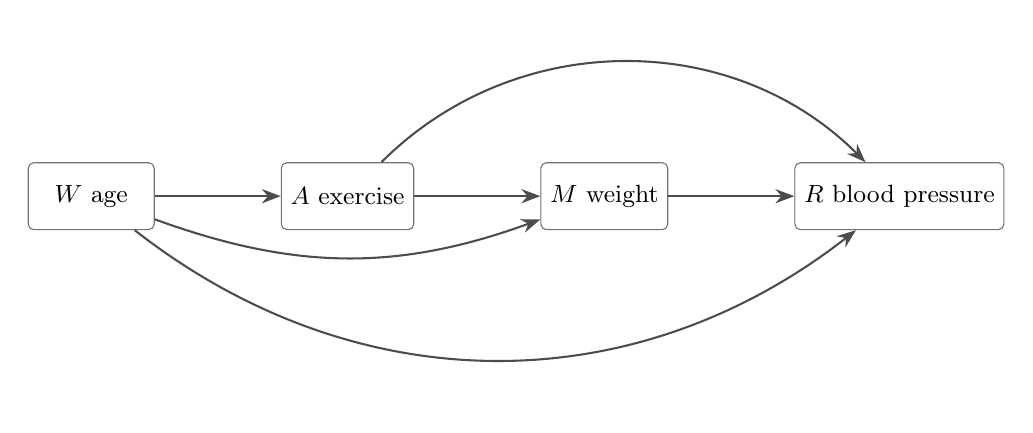
\begin{tikzpicture}[every node/.style={transform shape}]
  \node[defaultnode] (w) {$W$ age};
  \node[defaultnode, right=16mm of w] (a) {$A$ exercise};
  \node[defaultnode, right=16mm of a] (m) {$M$ weight};
  \node[defaultnode, right=16mm of m] (r) {$R$ blood pressure};
  \draw[normaledge] (w) -- (a);
  \draw[normaledge] (a) -- (m);
  \draw[normaledge] (m) -- (r);
  \draw[normaledge] (a) to[bend left=45] (r);
  \draw[normaledge] (w) to[bend right=20] (m);
  \draw[normaledge] (w) to[bend right=38] (r);
\end{tikzpicture}}
\caption{The running example's full causal graph (ECM), reproduced from
handout \S0: every earlier feature is drawn as a direct cause of every later
one (age $\to$ exercise, weight, blood pressure; exercise $\to$ weight,
blood pressure; weight $\to$ blood pressure).}
\label{fig:ecm-base}
\end{figure}

\subsection{The PDP, and why it isn't causally valid}

\textbf{PDP} \reusetag{Friedman 2001}: for each $a$, set everyone's exercise
to $a$, \emph{keep other features as recorded}, average predictions.
Problem: it silently holds weight and blood pressure fixed --- not what
would actually happen if someone exercised more. It answers ``what if only
exercise changed and nothing downstream reacted,'' rarely the causal
question actually wanted.

\medskip
\noindent\textbf{Formally} (Molnar's IML book, ch.~19, following
\reusetag{Friedman 2001}): split all the features the model uses into the
one(s) being plotted, $x_S$, and everything else, $X_C$ ($S$ and $C$
partition every feature $f$ takes as input). The partial dependence
function is
\begin{equation}
\hat f_S(x_S) \;=\; \mathbb{E}_{X_C}\big[\hat f(x_S, X_C)\big]
\;=\; \int \hat f(x_S, X_C)\, dP(X_C).
\label{eq:pdp-def}
\end{equation}
\noindent\textit{In words:} freeze the feature(s) you care about at the
value $x_S$ you want to plot on the $x$-axis, then average the model's
prediction over every possible value the \emph{other} features $X_C$ could
take, weighted by how often that combination actually occurs
($dP(X_C)$ is the real-world distribution of $X_C$). That gives one number
for that $x_S$; repeating it across a range of $x_S$ traces out the curve.

\medskip
\noindent\textbf{Why an integral, not a sum? --- the math one level down.}
$\mathbb{E}_{X_C}[\cdot]$ always means ``probability-weighted average,'' but
what that average looks like as a formula depends on whether $X_C$ is
discrete or continuous.

If $X_C$ could only take finitely many values $c_1,\dots,c_K$ (say, weight
rounded to the nearest kilogram), the weighted average would be an
ordinary sum:
$$\mathbb{E}_{X_C}[\hat f(x_S,X_C)] \;=\; \sum_{k=1}^K \hat f(x_S,c_k)\,
P(X_C=c_k).$$
But weight and blood pressure are \emph{continuous} --- they can take any
real value on a range, so there are infinitely many possible values, and
the probability of hitting any \emph{one exact} value is $0$ (e.g.\
$P(\text{weight}=71.3428\ldots\text{kg exactly})=0$; only \emph{intervals}
of values have positive probability). ``Multiply by $P(X_C=c_k)$ and sum''
breaks down here --- every term would be $0 \times (\text{something})$.

The fix is the same one ordinary calculus uses to define area under a
curve. Probability for a continuous variable is described by a
\textbf{density} $p(x_C)$, where $P(a\le X_C\le b)=\int_a^b p(x_C)\,dx_C$
(a density is a \emph{rate} --- probability per unit of $x_C$ --- not a
probability itself, which is why it's allowed to exceed $1$). Chop the
range of $X_C$ into thin slices of width $\Delta$; on each slice $X_C$ is
approximately discrete, landing in that slice with probability
$\approx p(x_C)\Delta$, so the weighted average over all the slices is
$$\sum_k \hat f(x_S,x_C^{(k)})\, p(x_C^{(k)})\, \Delta
\;\xrightarrow[\ \Delta\to 0\ ]{}\;
\int \hat f(x_S,x_C)\, p(x_C)\, dx_C.$$
That limit --- summing over infinitely many, infinitely thin slices --- is
exactly what an integral sign \emph{means}. It's the same idea as ``area
under a curve is the limit of a sum of thin rectangles'' from a first
calculus course, just with $\hat f(x_S,x_C)\,p(x_C)$ playing the role of
the curve's height.

\emph{Why $dP(X_C)$ instead of $p(x_C)\,dx_C$?} Writing $dP(X_C)$ is a
deliberate generalization: it means ``weighted by however probability is
actually spread out,'' without committing to whether $X_C$ is discrete,
continuous, or a mix. When $X_C$ is continuous, $dP(X_C) = p(x_C)\,dx_C$;
when it's discrete, $\int(\cdot)\,dP(X_C)$ collapses back into the ordinary
sum $\sum_k(\cdot)\,P(X_C{=}c_k)$ above --- one symbol covers both cases,
which is why $P(dw)$ in the notation table (\S\ref{sec:notation}) got the
same ``integrate or sum, whichever applies'' description.

\textbf{Where did $p(x_C^{(k)})\,\Delta$ go in the Monte Carlo sum below?}
Eq.~\eqref{eq:pdp-mc} is $\frac1n\sum_i \hat f(x_S,x_C^{(i)})$ --- no density,
no $\Delta$, every row weighted equally by $1/n$. That's not a different
formula from the slice-sum above; the density weight is still there, just
hidden inside \emph{which points you're summing over}. Here's the
derivation, one step at a time.

\begin{enumerate}
  \item Go back to the fixed grid of slices from before, spaced $\Delta$
    apart, with representative points $x_C^{(1)},x_C^{(2)},\dots$ --- these
    are evenly-spaced, chosen \emph{by you}, regardless of where real data
    lives. That's why each one needed an explicit
    $p(x_C^{(k)})\,\Delta$ multiplier: a grid point in a crowded region of
    the population and a grid point in a near-empty region get exactly one
    term each on the same grid, so probability has to be bolted on by hand
    to tell them apart.
  \item Now overlay your actual dataset on that same grid. Let $N_k$ be the
    number of your $n$ rows whose $x_C^{(i)}$ lands in slice $k$. Group the
    raw (unweighted) sum by which slice each row falls into --- $\hat f$
    barely changes across one thin slice, so every row in slice $k$
    contributes almost the same value, $\hat f(x_S,x_C^{(k)})$:
    $$\sum_{i=1}^n \hat f(x_S,x_C^{(i)}) \;\approx\;
    \sum_k N_k\,\hat f(x_S,x_C^{(k)}).$$
  \item Divide both sides by $n$:
    $$\frac1n\sum_{i=1}^n \hat f(x_S,x_C^{(i)}) \;\approx\;
    \sum_k \underbrace{\frac{N_k}{n}}_{\text{share of your data in slice }k}
    \hat f(x_S,x_C^{(k)}).$$
  \item This is the step that answers the question. $N_k/n$ is the
    \emph{empirical} fraction of your dataset that happens to land in
    slice $k$. If your dataset rows are a representative sample of the
    population (each one drawn from the true distribution of $X_C$), the
    Law of Large Numbers says that fraction converges, as $n$ grows, to the
    slice's \emph{true} probability --- which is exactly what a density
    means:
    $$\frac{N_k}{n} \;\xrightarrow[n\to\infty]{}\; P(X_C\in\text{slice }k)
    \;\approx\; p(x_C^{(k)})\,\Delta.$$
\end{enumerate}
So $p(x_C^{(k)})\,\Delta$ didn't disappear --- it's sitting inside $N_k/n$.
A crowded region of the population (high $p$) automatically contributes
\emph{many} rows to your dataset, so it automatically gets many terms in
the plain, unweighted sum; a rare region contributes few rows and few
terms. The multiplying-by-density step and the counting-more-rows-there
step are doing the identical job --- multiplying explicitly \emph{and}
sampling proportionally to density would double-count the same weighting.
Concretely: 10 people in your data with weight $\approx 70$kg contribute
10 near-identical terms to the raw average, automatically giving that
weight bracket $10\times$ the say of a bracket only 1 person has ---
that \emph{is} the density weighting, just paid for in row-count instead
of in an explicit multiplier. (This relies on the dataset actually being
representative of the population you want the curve to describe --- the
same ``which reference population'' issue flagged in \S\ref{sec:scope}.)

Putting the two limits together --- $\Delta\to 0$ (arbitrarily fine
slices) and $n\to\infty$ (arbitrarily large data) --- turns the slice-sum
into the exact integral, which is why Eq.~\eqref{eq:pdp-mc} is called an
\emph{estimator of} Eq.~\eqref{eq:pdp-def} rather than a separate
definition: same target, approached by letting real data stand in for the
unknown true distribution.

You can't literally integrate over the true, unknown distribution of
$X_C$, so in practice $\hat f_S$ is estimated by \textbf{Monte Carlo
averaging} over the dataset you actually have:
\begin{equation}
\hat f_S(x_S) \;=\; \frac{1}{n}\sum_{i=1}^n \hat f\big(x_S,\, x_C^{(i)}\big).
\label{eq:pdp-mc}
\end{equation}
\noindent\textit{In words:} go through every row $i$ in your dataset, one
at a time. For each row, swap in the fixed value $x_S$ for the feature(s)
you're plotting, but keep that \emph{same row's own, real, observed}
values for every other feature ($x_C^{(i)}$ --- the ``$(i)$'' means ``as
recorded for individual $i$,'' not a made-up value). Run the model once
per row under this swap, then average all $n$ of the resulting
predictions. ``Monte Carlo'' here just means: instead of doing the exact
integral in Eq.~\eqref{eq:pdp-def} (impossible, since you don't know the
true distribution $P(X_C)$), approximate it by an average over samples you
actually have --- your dataset itself stands in for that unknown
distribution, and the approximation gets better the more rows you average
over.

This is exactly the same computation as averaging every individual's ICE
(individual conditional expectation) curve at that $x_S$ --- a PDP curve
\emph{is}, by construction, the pointwise mean of all the ICE curves in
the dataset. And it's precisely the operation already described above in
words (``set everyone's exercise to $a$, keep other features as
recorded, average predictions''): Eq.~\eqref{eq:pdp-mc} is that sentence
written as a formula, with $S=\{A\}$ (exercise) and $C=\{M,R\}$ (weight,
blood pressure) in the running example.

\medskip
\noindent\textbf{A fully worked example, with numbers.} Suppose the
dataset has just $n=5$ people (a toy size, purely so every row can be
written out by hand), and a toy model
$$\hat f(A,M,R) \;=\; 100 - 2A + 0.3M + 0.4R$$
predicting a cardiovascular risk score from (exercise hrs/week $A$,
weight kg $M$, blood pressure $R$) --- a made-up linear formula, invented
only so the arithmetic below is checkable by hand; a real $\hat f$ would
be some fitted ML model with no such closed form.

\begin{table}[h]
\centering
\begin{tabular}{@{}cccc@{}}
\toprule
$i$ & $A_i$ (real) & $M_i$ (real) & $R_i$ (real) \\
\midrule
1 & 2 & 70 & 120 \\
2 & 5 & 65 & 110 \\
3 & 0 & 90 & 140 \\
4 & 3 & 75 & 125 \\
5 & 1 & 85 & 135 \\
\bottomrule
\end{tabular}
\caption{Toy dataset, $n=5$ people, each with their own recorded
$(A_i,M_i,R_i)$.}
\label{tab:pdp-toy}
\end{table}

To compute $\hat f_S(5)$ --- ``what would average predicted risk be if
\emph{everyone} exercised 5 hrs/week'' --- Eq.~\eqref{eq:pdp-mc} says: take
each row in Table~\ref{tab:pdp-toy}, replace $A_i$ with the fixed value
$5$, keep that same row's own $M_i,R_i$ completely untouched, run
$\hat f$, then average all 5 results:

\begin{table}[h]
\centering
\begin{tabular}{@{}ccl@{}}
\toprule
$i$ & $(x_S,\,x_C^{(i)}) = (5,\ M_i,\ R_i)$ & $\hat f(5,M_i,R_i)$ \\
\midrule
1 & $(5,\ 70,\ 120)$ & $100-10+21+48=159.0$ \\
2 & $(5,\ 65,\ 110)$ & $100-10+19.5+44=153.5$ \\
3 & $(5,\ 90,\ 140)$ & $100-10+27+56=173.0$ \\
4 & $(5,\ 75,\ 125)$ & $100-10+22.5+50=162.5$ \\
5 & $(5,\ 85,\ 135)$ & $100-10+25.5+54=169.5$ \\
\bottomrule
\end{tabular}
\caption{The 5 terms actually being averaged in Eq.~\eqref{eq:pdp-mc} at
$x_S=5$. Column 1 (exercise) is the same fixed $5$ in every row --- the
``freeze $x_S$'' part. Weight and blood pressure differ row by row ---
each person's own, untouched $x_C^{(i)}$.}
\label{tab:pdp-toy-eval}
\end{table}

$$\hat f_S(5) \;=\; \frac{159.0+153.5+173.0+162.5+169.5}{5}
\;=\; \frac{817.5}{5} \;=\; 163.5.$$

\noindent\textit{In words:} we are averaging over \textbf{5 numbers, one
per person in the dataset} --- not over 5 possible values of exercise, and
not over some abstract population. Person 3, who in reality never
exercises at all ($A_3=0$, Table~\ref{tab:pdp-toy}), still contributes a
term to this average: their \emph{predicted risk in a pretend world where
they exercised 5 hrs/week but kept their actual weight and blood
pressure} (173.0 --- the single highest of the five, driven entirely by
their real $M_3=90,R_3=140$, since $A$ is fixed at $5$ for every row
here, exercise contributes nothing to the differences between rows).
Repeating the same 5 rows with $x_S=0$ instead of $5$ gives
$\hat f_S(0)=173.5$ instead --- a different final number, because only
column 1 changed while the 5 real $(M_i,R_i)$ pairs stayed exactly the
same. That's the entire mechanism behind \emph{one point} of the PDP
curve; repeating this 5-row average once per value of $a$ traces out the
whole curve.

\textbf{The independence assumption, made concrete.} Eq.~\eqref{eq:pdp-mc}
pairs the fixed $x_S=a$ with \emph{every} row's own $x_C^{(i)}$, including
rows whose real exercise level was nothing like $a$. That's fine only if
exercise and (weight, blood pressure) are unrelated --- but they aren't
(that's the whole running example). Concretely, in
Table~\ref{tab:pdp-toy-eval}: Person 3 really never exercises
($A_3=0$) and really carries a high weight/BP profile ($M_3=90,R_3=140$)
--- plausibly \emph{because} they don't exercise. Eq.~\eqref{eq:pdp-mc}
still uses their $(M_3,R_3)$ as a stand-in for ``someone who exercises 5
hrs/week,'' as if that weight/BP combination were a realistic thing to see
at high exercise, when in this population it may never actually occur
there.
This is the same mechanism as the confounding problem in
\S\ref{sec:background} --- it's why the PDP ``isn't causally valid'' named
in this subsection's title, and it's exactly what the CDP framework below
is built to fix.

\bigskip
\noindent\textbf{Aside: PDP-based feature importance}
\reusetag{Greenwell, Boehmke \& McCarthy 2018}. Not part of the CDP
framework itself, but built directly on the PDP curve just defined, and
worth having on hand since ``does this curve actually vary, or is it
flat?'' is a question that comes back repeatedly later.

\emph{The idea in one sentence:} a flat PDP curve means the feature barely
changes the prediction (not important); a curve that swings up and down a
lot means the feature matters a lot (important). Feature importance turns
``how much does the curve vary'' into a single number.

\textbf{Numerical features.} Evaluate the PDP curve $\hat f_S$ at its $K$
\emph{unique observed values} $x_S^{(1)},\dots,x_S^{(K)}$ (literally every
distinct value the feature actually takes in the dataset, not an
arbitrary grid), then measure how spread out those $K$ curve heights are
around their own average:
\begin{equation}
I(x_S) \;=\; \frac{1}{K-1}\sum_{k=1}^K
\left(\hat f_S\big(x_S^{(k)}\big) - \frac{1}{K}\sum_{k=1}^K
\hat f_S\big(x_S^{(k)}\big)\right)^{\!2}.
\label{eq:pdp-importance-numeric}
\end{equation}
\noindent\textit{In words:} the inner term
$\frac1K\sum_k \hat f_S(x_S^{(k)})$ is just the \emph{average height} of
the curve across its $K$ points --- the flat reference line you'd see if
the feature had zero effect. For each point, subtract that average and
square the result: a point on a flat curve sits close to the average, so
this is close to $0$; a point far from the average (the curve is
swinging there) gives a large squared number. Add up all $K$ squared
deviations and divide by $K-1$. This is nothing more exotic than the
ordinary \textbf{sample variance formula}
($s^2=\frac1{n-1}\sum(y_i-\bar y)^2$, same $K-1$ denominator for the same
reason) applied to the $K$ curve heights instead of $K$ raw data points
--- ``importance'' here literally \emph{means} ``variance of the PDP
curve.''

\emph{Worked example, continuing the toy dataset above.} Since
$\hat f_S(a) = 100-2a+73.5 = 173.5-2a$ in the running toy (the average of
$0.3M_i+0.4R_i$ over the 5 people works out to $73.5$), the $K=5$ unique
real exercise values $\{0,1,2,3,5\}$ give curve heights
$\{173.5,\,171.5,\,169.5,\,167.5,\,163.5\}$, averaging to $169.1$. Squared
deviations: $4.4^2,2.4^2,0.4^2,(-1.6)^2,(-5.6)^2 =
19.36,\,5.76,\,0.16,\,2.56,\,31.36$, summing to $59.2$. So
$I(A) = 59.2/4 = 14.8$. If exercise instead had \emph{no} effect on
$\hat f$ at all, all 5 curve heights would be identical, every squared
deviation would be $0$, and $I(A)$ would come out exactly $0$ --- that's
the whole point of the measure.

\textbf{Categorical features.} Categories don't sit on a number line, so
``deviation from the mean'' isn't quite the natural notion; a cruder,
more robust measure is used instead --- the \textbf{range rule}:
\begin{equation}
I(X_S) \;=\; \frac{\max_k\big(\hat f_S(x_S^{(k)})\big)
- \min_k\big(\hat f_S(x_S^{(k)})\big)}{4}.
\label{eq:pdp-importance-categorical}
\end{equation}
\noindent\textit{In words:} take the PDP's highest value across the $K$
categories, subtract its lowest value, divide by $4$. \emph{Why divide by
$4$?} A rule of thumb borrowed from the normal distribution: about $95\%$
of a normal distribution's mass sits within $\pm 2$ standard deviations of
its mean --- a band $4$ standard deviations wide. So if all you know is a
variable's range (max$-$min) and want a rough guess at its standard
deviation, range$/4$ is a reasonable back-of-envelope estimate
($\text{range}\approx 4\sigma \Rightarrow \sigma\approx
\text{range}/4$). It's deliberately crude and typically
\emph{underestimates} the true spread --- but with only a handful of
categories ($K$ small), there's little basis for a real variance estimate
anyway, which is exactly why the cruder range-based version replaces
Eq.~\eqref{eq:pdp-importance-numeric} here.

\emph{Worked example (toy, illustrative numbers, following Molnar's own
season/bike-rental example):} PDP-predicted bike rentals by season,
Spring$=150$, Summer$=180$, Fall$=165$, Winter$=90$. Range
$=180-90=90$, so $I(\text{season}) = 90/4 = 22.5$.

\textbf{Two things this measure is \emph{not}.} (1) It only sees the
feature's \emph{main effect} --- the shape of its own PDP curve --- and
is blind to \emph{interactions}: a feature that matters only by
interacting with another feature (e.g.\ flipping sign depending on a
second feature's value, the heterogeneous-effects problem from the
recall questions above) can have a nearly flat, low-$I$ PDP curve while
still being genuinely important to the model --- permutation feature
importance would catch that; this measure would miss it. (2) It weights
every \emph{unique value} equally, regardless of how many rows share it
--- a value only one person in the dataset has counts exactly as much as
a value shared by hundreds, unlike the PDP curve itself
(Eq.~\eqref{eq:pdp-mc}), which already weights by how common a value's
neighborhood is via the Monte Carlo average.

\subsection{The fix: use the ECM to define ``changing \texorpdfstring{$A$}{A}''}

\textbf{ECM} = ``explanatory causal model'' --- the analyst's DAG over the
\emph{features}. It is an assumption brought to the explanation, not a claim
verified by the model. Given an ECM, there is more than one way to ask ``how
does output depend on $A$'' --- there are (at least) four, depending on
whether downstream features are allowed to respond:

\begin{table}[h]
\centering
\begin{tabular}{@{}p{2.6cm}p{5.2cm}p{5.6cm}@{}}
\toprule
\textbf{Plot} & \textbf{Question} & \textbf{In the running example} \\
\midrule
TDP (total) & set $A=a$; let everything downstream respond &
  weight and BP move \\
NDDP (natural direct) & set $A=a$; hold downstream features at their
  \emph{natural} values & \textbf{this is exactly the PDP} (handout's
  Thm.\ 2.10) \\
NIDP (natural indirect) & keep your own $A$; move downstream features to
  where they'd be under $A=a$ & your exercise, but the weight/BP you'd have
  at exercise $a$ \\
PCDP (partially controlled) & set $A=a$ \emph{and} fix another feature &
  exercise $=a$, weight $=m$ \\
\bottomrule
\end{tabular}
\caption{The four named dependence plots.}
\label{tab:four-plots}
\end{table}

The genuinely new fact worth internalizing early: $\mathbf{NDDP = PDP}$. The
plot everyone already uses is a special case of this framework --- the
``direct effect only'' member of the family, not a separate method.

\subsection{Constructed outcome --- the trick that makes this identifiable}

Treat the model's output as a variable: $Y^* = f(X)$. Then the
\textbf{average TDP is a plain back-door adjustment}:
\begin{equation}
  \theta(a) \;=\; E[f(X) \mid \operatorname{do}(A=a)]
  \;=\; E_W\big[\, E[Y^* \mid A=a, W] \,\big], \qquad W = \text{parents of } A.
  \label{eq:tdp-backdoor}
\end{equation}
\emph{In words:} the average model output you'd get from forcing everyone
to exercise level $a$ ($\theta(a)$, left-hand side) equals a two-step
average on the right: first, within each age group $w$, average the
model's prediction over the people who actually exercise at level $a$
(inner $E[Y^*\mid A=a,W]$); then average those age-group numbers together
using the real population mix of ages ($E_W[\cdot]$) --- the same
``average over the marginal, not the conditional'' move as
Eq.~\ref{eq:backdoor}, now applied to the model's output instead of a raw
outcome.
\reusetag{Pearl 2009, Thm.\ 3.2.2; Zhao \& Hastie 2021 (theorem)}; \newtag~is
what this implies specifically for CDPs. The equations for weight and blood
pressure are never needed: $\operatorname{do}(A=a)$ leaves the parents'
distribution alone and leaves every downstream conditional given $(a,w)$
alone. This is \emph{why} \S\ref{sec:identification} can get away with only
needing the parents plus a ``reduced form,'' not the full fitted ECM.

\subsection{The picture that organizes the whole family}

\reusetag{Shpitser \& Tchetgen Tchetgen 2016} Add the model's output $\hat Y$
to the graph as a child of every feature. Then TDP/PCDP are ordinary node
interventions ($\operatorname{do}(A=a)$, $\operatorname{do}(A=a,C=c)$), while
NDDP/NIDP are \textbf{edge} interventions (set $a$ on the arrow into $\hat
Y$ only, vs.\ on the arrows into the child features only). Normally, one
node ``acting two ways at once'' needs cross-world assumptions data cannot
check --- but here $\hat Y = f(X)$ is a \emph{known function}, so nothing
cross-world is actually invoked. That is the structural reason NDDP reduces
to an ordinary average (the PDP) and NIDP reduces to an ordinary
single-world quantity (\S\ref{sec:identification}).

\begin{figure}[htbp]
\centering
\begin{subfigure}[t]{0.47\textwidth}
\centering
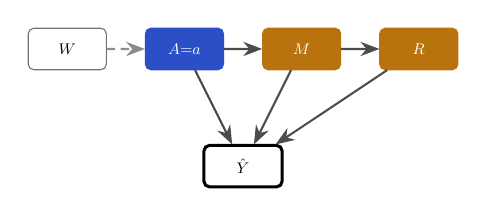
\begin{tikzpicture}[scale=0.62, every node/.style={transform shape}]
  \node[defaultnode] (w) at (0,1.6) {$W$};
  \node[accentnode] (a) at (2.4,1.6) {$A{=}a$};
  \node[respondnode] (m) at (4.8,1.6) {$M$};
  \node[respondnode] (r) at (7.2,1.6) {$R$};
  \node[targetnode] (y) at (3.6,-0.8) {$\hat Y$};
  \draw[severededge] (w) -- (a);
  \draw[normaledge] (a) -- (m);
  \draw[normaledge] (m) -- (r);
  \draw[normaledge] (a) -- (y);
  \draw[normaledge] (m) -- (y);
  \draw[normaledge] (r) -- (y);
\end{tikzpicture}
\caption{TDP --- total: \texttt{do(A=a)} cuts the arrow into $A$; $M$ and $R$
respond through the normal mechanism; everything reaches $\hat Y$.}
\label{fig:tdp}
\end{subfigure}
\hfill
\begin{subfigure}[t]{0.47\textwidth}
\centering
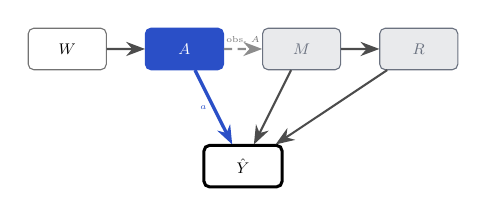
\begin{tikzpicture}[scale=0.62, every node/.style={transform shape}]
  \node[defaultnode] (w) at (0,1.6) {$W$};
  \node[accentnode] (a) at (2.4,1.6) {$A$};
  \node[naturalnode] (m) at (4.8,1.6) {$M$};
  \node[naturalnode] (r) at (7.2,1.6) {$R$};
  \node[targetnode] (y) at (3.6,-0.8) {$\hat Y$};
  \draw[normaledge] (w) -- (a);
  \draw[severededge] (a) -- (m) node[midway, above, font=\tiny, text=black!55] {obs.\ $A$};
  \draw[normaledge] (m) -- (r);
  \draw[accentedge] (a) -- (y) node[midway, left, font=\tiny, text=accentc] {$a$};
  \draw[normaledge] (m) -- (y);
  \draw[normaledge] (r) -- (y);
\end{tikzpicture}
\caption{NDDP $=$ PDP --- natural direct: only the arrow into $\hat Y$
carries $a$; $M$ and $R$ are left at their natural (recorded) values.}
\label{fig:nddp}
\end{subfigure}

\medskip

\begin{subfigure}[t]{0.47\textwidth}
\centering
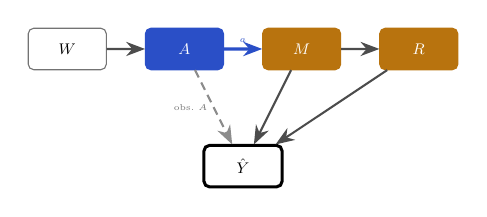
\begin{tikzpicture}[scale=0.62, every node/.style={transform shape}]
  \node[defaultnode] (w) at (0,1.6) {$W$};
  \node[accentnode] (a) at (2.4,1.6) {$A$};
  \node[respondnode] (m) at (4.8,1.6) {$M$};
  \node[respondnode] (r) at (7.2,1.6) {$R$};
  \node[targetnode] (y) at (3.6,-0.8) {$\hat Y$};
  \draw[normaledge] (w) -- (a);
  \draw[accentedge] (a) -- (m) node[midway, above, font=\tiny, text=accentc] {$a$};
  \draw[normaledge] (m) -- (r);
  \draw[severededge] (a) -- (y) node[midway, left, font=\tiny, text=black!55] {obs.\ $A$};
  \draw[normaledge] (m) -- (y);
  \draw[normaledge] (r) -- (y);
\end{tikzpicture}
\caption{NIDP --- natural indirect: the arrow into $M$ carries $a$ (so $M,R$
move to their counterfactual values); the direct arrow into $\hat Y$ keeps
the observed $A$. Identified as Fulcher et al.'s ``bridge mean.''}
\label{fig:nidp}
\end{subfigure}
\hfill
\begin{subfigure}[t]{0.47\textwidth}
\centering
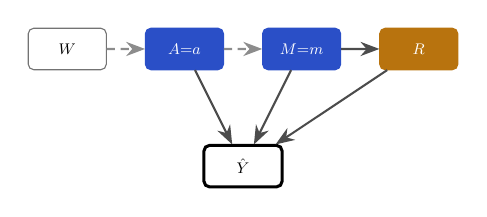
\begin{tikzpicture}[scale=0.62, every node/.style={transform shape}]
  \node[defaultnode] (w) at (0,1.6) {$W$};
  \node[accentnode] (a) at (2.4,1.6) {$A{=}a$};
  \node[accentnode] (m) at (4.8,1.6) {$M{=}m$};
  \node[respondnode] (r) at (7.2,1.6) {$R$};
  \node[targetnode] (y) at (3.6,-0.8) {$\hat Y$};
  \draw[severededge] (w) -- (a);
  \draw[severededge] (a) -- (m);
  \draw[normaledge] (m) -- (r);
  \draw[normaledge] (a) -- (y);
  \draw[normaledge] (m) -- (y);
  \draw[normaledge] (r) -- (y);
\end{tikzpicture}
\caption{PCDP --- partially controlled: \texttt{do(A=a,M=m)} cuts both
incoming arrows; $R$ still responds to the fixed $M$; both $a$ and $m$ reach
$\hat Y$.}
\label{fig:pcdp}
\end{subfigure}
\caption{The four dependence plots as different interventions on the same
explanatory causal model. \emph{Simplified for legibility}: the full ECM
(Figure~\ref{fig:ecm-base}, handout \S0) also has direct edges $W\to M$,
$W \to R$, $A \to R$ among the features, and --- since $\hat Y$ is a child
of every feature --- a direct $W \to \hat Y$ edge; all four are omitted here
so the direct/indirect mechanism stays readable. Blue $=$ set to the
counterfactual value; amber $=$ responds/recomputed; gray $=$ kept at its
natural (recorded) value; dashed $=$ edge severed, or carrying the natural
value instead of $a$.}
\label{fig:four-plots}
\end{figure}

\noindent\textbf{Legend:}
\begin{itemize}[leftmargin=1.6em, itemsep=2pt]
  \item[\textcolor{accentc}{$\bullet$}] set to the counterfactual value
  \item[\textcolor{respondc}{$\bullet$}] responds / recomputed
  \item[\textcolor{naturalc}{$\bullet$}] kept at natural (recorded) value
  \item[-----] active edge (solid)
  \item[- - -] severed edge, or an edge carrying the natural value instead
    of $a$
\end{itemize}

\begin{quote}
\textbf{Direct + indirect $\neq$ total.} \newtag, modest.
\[
  \theta(a) - B \;=\; [\mathrm{NDDP}(a) - B] + [\mathrm{NIDP}(a) - B] + J(a),
\]
\emph{In words:} take how far the total curve is from the overall average
prediction ($\theta(a) - B$, left side). You might expect that gap to split
cleanly into ``how much of it is the direct effect'' plus ``how much of it
is the indirect effect'' (the two bracketed terms on the right). It doesn't,
in general --- there's a leftover piece $J(a)$ that has to be added to make
the two sides match, and $J(a)$ is exactly zero only in the special case
where $f$ treats $A$ and the downstream features additively (no
interaction between them).

Here $B$ is the average prediction and $J$ is an interaction remainder that
vanishes only when $f$ is additive in $A$ and the downstream features. Toy
counterexample: $A \sim \mathrm{Bern}(p)$, $R(a) = a$, $f = a \cdot r$; the
total contrast is $1$, but the direct and indirect contrasts are each only
$p$. \textbf{Don't assume direct $+$ indirect sums to total} --- $J$ should
be plotted alongside them, not ignored.
\end{quote}

\begin{openquestions}
  \item Work through why exactly the parents' distribution is untouched by
    $\operatorname{do}(A=a)$ --- is this just the definition of ``parents,''
    or does it need the ECM to have no unmeasured confounding among
    features?
  \item Read arXiv \S1--2 in full (the mentor's prescribed order has this
    \emph{before} rereading the handout) for the paper's own formal
    definitions, then compare notation to the handout's.
\end{openquestions}

\section{Identification: what each plot needs from the data}
\label{sec:identification}

\emph{Source: handout \S1.1. This is the intern-term paper's (``Paper A'')
first result. Status: skeleton from a first read.}

\subsection{The reduced form}

Let $R$ be the features other than $A$ and its parents $W$. Let
$Q(dr \mid a, w)$ be the conditional law of $R$ given $(A,W)$ --- the
\textbf{reduced form}. Crucially, this is \emph{learnable straight from
data} --- no ECM structural equations needed.

\subsection{Per-plot identification table}

\begin{table}[h]
\centering
\begin{tabular}{@{}p{2.1cm}p{4.4cm}p{3.6cm}p{3.4cm}@{}}
\toprule
\textbf{Plot} & \textbf{Population target} & \textbf{What it consumes} &
\textbf{Statistical character} \\
\midrule
TDP & $\int P(dw) \int Q(dr\mid a,w)\, f(a,w,r)$ & parents $+$ reduced form &
  AIPW; $\sqrt{n}$ at discrete levels \\
NDDP $=$ PDP & $E[f(a, X_{-A})]$ & \textbf{no causal nuisance at all} ---
  only $f$ and the reference distribution of $X_{-A}$ & sample mean of a
  known function; $\sqrt{n}$ at each $a$ \\
NIDP & $\int P(da', dw) \int Q(dr\mid a,w)\, f(a', w, r)$ & parents $+$
  reduced form $+$ law of $A$ given $W$ & its own influence function;
  $\sqrt{n}$ at discrete levels \\
PCDP & needs the graph \emph{inside} $R$ & more than the reduced form (two
  graphs with the same data give different answers) & g-formula \\
\bottomrule
\end{tabular}
\caption{Identification of each named plot (handout \S1.1).}
\label{tab:identification}
\end{table}

\emph{Reading the three dense formulas in words:} TDP's
$\int P(dw) \int Q(dr\mid a,w)\, f(a,w,r)$ says --- go age group by age
group ($\int P(dw)$, weighting by how common each age group actually is);
within each age group, average over what weight-and-blood-pressure values
typically go with exercise level $a$ there ($\int Q(dr\mid a,w)$, the
reduced form); then plug each $(a,w,r)$ combination into the model $f$ and
average. NIDP's formula is almost identical but starts by also averaging
over exercise levels $a'$ drawn the way they actually occur for each age
group ($\int P(da',dw)$) before asking what downstream values go with the
\emph{target} level $a$ --- that's the ``your own exercise, but their
downstream values'' mixing. NDDP's $E[f(a,X_{-A})]$ is the simplest: just
plug the fixed value $a$ in for exercise, leave every other feature exactly
as recorded in the data, run it through $f$, and average --- no age
groups, no reduced form, nothing learned about causal structure at all.

\textbf{Takeaway to hold onto:} three of the four named plots (TDP, NDDP,
NIDP) need \emph{only} the parents of $A$ plus one reduced form --- fitting
every equation of the ECM is never required. Only PCDP needs the internal
graph structure of $R$. This is what makes ``adjustment''
(\S\ref{sec:estimation}) a real alternative to ``propagation''
(\S\ref{sec:propagation}) for three of the four plots.

\subsection{NIDP \texorpdfstring{$=$}{=} a known bridge mean (reuse, not a new discovery)}

\reusetag{Fulcher, Shpitser, Marealle \& Tchetgen Tchetgen 2020, JRSSB}
``Your own $A$, but the downstream values you'd have had under $A=a$'' is
exactly their \textbf{bridge mean} $\Psi(a) = E[Y(A, Z(a))]$ from the
population-intervention indirect-effect literature ($Z=$ downstream
features, $Y=f$) --- in words, plug each person's \emph{own actual}
exercise level ($A$, not $a$) into the model, but pair it with the
downstream feature values ($Z(a)$) they \emph{would have had} under the
hypothetical exercise level $a$, then average over everyone. It mixes one
real, observed input with one counterfactual input for the same person.
Their Lemma~1 gives the formula, their Theorem~1 gives its
influence function (one term drops out here because $Y^*=f(X)$ is
\emph{deterministic}, not noisy), and their doubly-robust estimator applies
directly.

What's \newtag~here specifically: recognizing the published NIDP \emph{is}
this object, that the covariate set reduces to just the parents of $A$, and
the simplifications that follow from $f$ being a known function rather than
an unknown outcome-generating process. Caveat: handled for
\textbf{discrete $A$ only} this term --- continuous-$A$ NIDP needs its own
theory.

\subsection{Direct \texorpdfstring{$+$}{+} indirect \texorpdfstring{$\neq$}{!=} total}

\newtag, modest. With $B$ the average prediction:
\[
  \theta(a) - B \;=\; [\mathrm{NDDP}(a) - B] + [\mathrm{NIDP}(a) - B] + J(a),
\]
(in words: the total curve's distance from the average, on the left, isn't
simply the direct effect's distance plus the indirect effect's distance ---
there's a leftover term $J(a)$ needed to make the two sides balance; see
\S\ref{sec:bigpicture} for the full walkthrough). $J$ is an interaction remainder --- it vanishes only when $f$ is additive in
$a$ and the downstream features. Toy counterexample: $A \sim \mathrm{Bern}(p)$,
$R(a)=a$, $f = a\cdot r$: the total contrast is $1$, but the direct and
indirect contrasts are each only $p$. \textbf{Don't assume direct $+$
indirect sums to total} --- $J$ should be plotted alongside them, not
ignored.

\begin{openquestions}
  \item Why does PCDP specifically need the graph \emph{inside} $R$, when
    TDP/NDDP/NIDP don't need any equations at all? (Intuition: fixing an
    intermediate feature ``cuts'' a path in a way sensitive to which
    downstream variable causes which --- worth confirming with a toy SCM.)
  \item Verify \S1.1's table by exact enumeration in toy SCMs --- handout
    \S1.9 marks this as intern-feasible / light supervision (\feasyes).
    Good first task.
\end{openquestions}

\section{Estimation: AIPW, cross-fitting, and which covariates to adjust for}
\label{sec:estimation}

\emph{Source: handout \S1.2--1.3. Status: skeleton from a first read.}

\subsection{Estimating one level, discrete \texorpdfstring{$A$}{A} (\S1.2, mostly REUSE)}

Three classical estimators (Robins/Rotnitzky/Zhao 1994; Hahn 1998):
regression (regress $Y^*$ on $(A,Z)$, average), inverse-propensity
weighting, or \textbf{AIPW}, which combines both and is \emph{doubly
robust} --- consistent if \emph{either} piece is right:
\begin{equation}
  \hat\theta(a) \;=\; \frac{1}{n}\sum_{i=1}^n \left[
    \frac{\mathbf{1}(A_i=a)}{\hat\pi(a\mid Z_i)}\big(Y_i^* - \hat\mu(a,Z_i)\big)
    + \hat\mu(a,Z_i) \right].
  \label{eq:aipw}
\end{equation}
\emph{In words, person by person:} start with the regression's best guess
for person $i$'s outcome if they'd had exercise level $a$, given their
covariates ($\hat\mu(a,Z_i)$ --- this term alone is used for everyone). Then,
\emph{only for the people who actually did exercise at level $a$}
($\mathbf{1}(A_i=a)$ switches this next part on or off), add a correction:
how far their real outcome was from that regression guess
($Y_i^* - \hat\mu(a,Z_i)$), inflated by how rare it was for someone with
their covariates to end up at exercise level $a$
($1/\hat\pi(a\mid Z_i)$ --- rarer means a bigger correction, since that
person is doing more work standing in for others like them). Average this
person-by-person quantity over everyone, and that's $\hat\theta(a)$. The
``doubly robust'' part: if $\hat\mu$ is wrong but $\hat\pi$ is right, the
correction term fixes it on average; if $\hat\pi$ is wrong but $\hat\mu$ is
right, the correction term is small anyway because the regression guess was
already good.

\textbf{Cross-fitting} \reusetag{Chernozhukov et al.\ 2018}: fit
$\hat\mu, \hat\pi$ on one data half, evaluate on the other, swap. This lets
flexible ML be used for the nuisance functions while still getting a valid
Wald interval $\hat\theta(a) \pm 1.96\,\widehat{\mathrm{se}}$, \emph{provided}
the two nuisance errors shrink fast enough \emph{jointly} (their product
must be $o_p(n^{-1/2})$). Cross-fitting removes a technical condition, not
the underlying accuracy requirement --- a common misreading to watch for.

\subsection{Which covariates \texorpdfstring{$Z$}{Z} to adjust for (\S1.3)}

\reusetag{Rotnitzky \& Smucler 2020}, \newtag~application. The parents $W$
are a \emph{valid} adjustment set but not necessarily the lowest-variance
one. Adding non-descendants of $A$ that help predict $Y^*$ lowers variance
without changing the answer (same logic as good covariates in a randomized
trial).

\textbf{Key result:} when $f$ uses all features, the set of \emph{all
non-descendants of $A$} is never worse than any other valid set in large
samples (among the adjustment estimators used here). Two practical facts:
\begin{enumerate}[label=(\alph*)]
  \item The \emph{population} positivity condition does not get harder ---
    because $P(a \mid \text{non-descendants}) = P(a \mid W)$ by the graph.
    What gets harder is \emph{fitting} a bigger regression in finite
    samples. So: \textbf{fit the propensity on $W$, fit the outcome
    regression on the larger set.}
  \item This result uses only the graph's \emph{arrows} --- never its
    equations. (The handout notes this was verified exhaustively on small
    graphs in the review --- a good sanity-check exercise to redo.)
\end{enumerate}

\begin{openquestions}
  \item Work through \emph{why} adding non-descendants can only help (not
    hurt) asymptotic variance --- is there a clean intuition beyond ``more
    relevant predictors of $Y^*$ reduce residual variance''?
  \item Handout \S1.9 marks ``cross-fitted AIPW at discrete levels; coverage
    on oracle testbed'' as intern-feasible / moderate supervision
    (\feasmod), and ``parents vs.\ efficient set (variance drop)'' likewise
    --- plausible first coding tasks once toy-SCM verification
    (\S\ref{sec:identification}) is done.
\end{openquestions}

\section{Continuous \texorpdfstring{$A$}{A}: bins first, curves second}
\label{sec:continuous}

\emph{Source: handout \S1.4. Status: skeleton from a first read.}

\subsection{Bins (primary target)}

At each bin $B_k$, report the fixed-weight average
$\psi_k = \int_{B_k} \theta(a)\, g_k(a)\, da$ --- in words, don't report the
true curve $\theta(a)$ at every single value of $a$ in the bin; instead,
report one number per bin, obtained by averaging $\theta(a)$ over all the
$a$-values inside that bin ($B_k$), using a weighting rule $g_k$ that's
written down \emph{before} looking at the data (e.g.\ ``just weight every
$a$-value in the bin equally''). Why fix the weight ahead of time rather
than use the observed distribution of $A$ inside the bin: weighting by the
observed distribution makes the target depend on the data law and adds a
term to the standard error. This is a regular, $\sqrt{n}$ target, estimated
by the same AIPW machinery (Eq.~\ref{eq:aipw}) with weight
$g_k(A)/\hat\pi(A\mid Z)$ --- and it does not depend on which valid $Z$ was
chosen (\S\ref{sec:estimation}).

\subsection{Smoothed curve --- two tiers}

\begin{itemize}
  \item \textbf{Smoothed curve (extension, supervisor-owned)}:
    $\theta_h = K_h * \theta$ at a declared bandwidth $h$ --- in words, the
    smoothed curve's value at a point is a local weighted average of the
    true curve $\theta$ near that point, where the kernel $K_h$ is the rule
    for how much weight nearby $a$-values get (points closer than the
    bandwidth $h$ count more, points farther away count less or not at
    all) --- kernel-weighted
    AIPW, bands via multiplier bootstrap. Works for \emph{any} $f$ ---
    important because a tree that splits on $A$ can make $\theta$ itself
    jumpy, and the ``smooth curve'' theory below assumes smoothness a jumpy
    $\theta$ doesn't have.
  \item \textbf{Smooth curve (secondary, if $\theta$ is actually smooth)}:
    cite Takatsu \& Westling's debiased local-linear estimator, or Semenova
    \& Chernozhukov's cross-fitted series estimator (its variance has an
    extra term that must not be dropped). Pseudo-outcome must be Kennedy's
    construction --- the naive ``$\hat\mu + (Y^*-\hat\mu)/\hat\pi$ regressed
    on $A$'' estimates the wrong thing (handout notes it was checked to be
    off by $0.9$ in a toy example --- a concrete trap to avoid
    reinventing).
\end{itemize}

\subsection{Bias policy}

\newtag~correction. Any uncorrected smoother at its best bandwidth has bias
as large as its standard error, so naive confidence bands
\textbf{under-cover}. The project's earlier prototype hit exactly this
(0.89 coverage instead of $\sim$0.95). Fix: debiasing, deliberate
undersmoothing, or report bands for $\theta_h$ itself rather than pretending
they are bands for the unsmoothed $\theta$.

\begin{openquestions}
  \item Handout marks the (primary) fixed-bin estimator as intern-feasible
    (\feasmod{} --- ``representer, bootstrap over a finite vector''). The
    smoothed curve is explicitly \feasno{} / not intern-feasible --- don't
    invest here without direction.
  \item Understand precisely why a data-dependent bin weight adds a
    standard-error term --- worth a small derivation.
\end{openquestions}

\section{Adjustment vs.\ propagation, and sensitivity analysis}
\label{sec:propagation}

\emph{Source: handout \S1.5--1.6. Status: skeleton from a first read.}

\subsection{Adjustment vs.\ propagation (\S1.5)}

\newtag~study. Four arms compared: parents only; the efficient covariate set
(\S\ref{sec:estimation}); an estimator exploiting the DAG's factorization;
and full \textbf{parametric propagation} (fit every ECM structural equation,
simulate --- what the \emph{original} CDP paper's method does).

Findings to reproduce/understand, not just quote:
\begin{itemize}
  \item A confounder living entirely \textbf{downstream} (e.g.\ between
    weight and blood pressure, independent of exercise) does \emph{not}
    invalidate the parent-adjustment formula for the \emph{total} curve ---
    the formula is right whether or not that confounder is drawn in the
    graph. It changes the data (and so the curve), but adjustment still
    recovers the right curve for whatever the data is. Propagation only
    inherits this if its fitted conditionals match the observational ones
    --- which holds \emph{exactly} for linear OLS (an algebraic identity:
    fitted path coefficients always compose to the reduced-form slope) but
    can fail for nonlinear $f$: a Gaussian propagation model can match the
    mean and variance exactly and \emph{still} get $E[f]$ wrong (handout
    cites a checked example: error $0.047$ with mean and variance exact).
    \textbf{Nonlinearity is where propagation's extra assumptions can
    bite.}
  \item When the ECM's parametric equations are correct, propagation can be
    \emph{more precise} and can extrapolate outside the region of data
    overlap --- but that should be declared as model-based extrapolation,
    not treated as free. Overlap is diagnosed via the \textbf{non-overlap
    ratio} \reusetag{Bao \& Schomaker 2026}.
  \item Whether exploiting the DAG's factorization can beat plain adjustment
    at all is answered by \reusetag{Rotnitzky \& Smucler 2020, Thm.\ 19}.
\end{itemize}

\subsection{Sensitivity analysis (\S1.6)}

Mostly \reusetag{Cinelli \& Hazlett 2020; nonparametric bounds: Chernozhukov,
Cinelli, Newey, Sharma \& Syrgkanis}, \newtag~framing. If an unmeasured $U$
affects $A$ \emph{and} a downstream feature that matters for $f$, it can
bias the adjusted curve (special cases: the bias cancels, or $U$ turns out
irrelevant to $f$). Uses \textbf{partial-$R^2$ sensitivity} to ask: how
strong would $U$ need to be to flip the \textbf{slope} (never the level ---
that depends on an arbitrary zero point), flatten the curve, or cross a
threshold?

Project-specific (\newtag) content: confounding parameterized \emph{per ECM
edge}, with an exact map to the standard Cinelli--Hazlett coordinates (the
``tipping strength'' is their robustness-value formula, just
reparameterized); bounds at each bin; benchmarking against observed
predictors; and cross-checking against the \S1.5 invariance result above.

\begin{openquestions}
  \item Handout marks ``propagation arm via DoWhy $+$ invariance
    demonstrations'' as intern-feasible / moderate (\feasmod) --- a
    plausible task once \S\ref{sec:identification}/\S\ref{sec:estimation}
    basics are solid.
  \item ``Robustness section: linear closed forms, planted confounders,
    tipping, benchmarking'' is intern-feasible / moderate (\feasmod), with
    binned Riesz bounds ``only if time allows'' --- i.e.\ a stretch goal,
    not baseline scope.
  \item Work the toy linear-OLS ``path coefficients compose to the
    reduced-form slope'' identity by hand for the running example graph.
\end{openquestions}

\section{Practical rules, and what this term's paper does \emph{not} claim}
\label{sec:scope}

\emph{Source: handout \S1.7--1.9, \S2. Status: skeleton from a first read.}

\subsection{Two cheap but important rules (\S1.7)}

\newtag, cheap, important.
\begin{enumerate}
  \item \textbf{Explanatory data must be held out.} $Y_i^* = f(X_i)$ on rows
    used to \emph{train} $f$ is not a fair sample of what $f$ does (a random
    forest nearly reproduces its own training outcomes). Draw every curve
    on rows the model never saw. Out-of-bag / cross-fitted predictions are
    predictions of \emph{different} models, not of $f$ itself --- don't
    substitute them.
  \item \textbf{Name the reference population.} The outer average is over
    some distribution of $W$; training cohort, held-out sample, and
    deployment population give genuinely different curves whenever the
    effect varies with $w$. This term's inference is all for the
    \emph{held-out sample's} population. Carrying a curve to a different
    population (``transport'') needs extra data and different formulas ---
    explicitly \textbf{out of scope} this term.
\end{enumerate}

\subsection{What Paper A does \emph{not} claim (\S1.8)}

Not claiming: that parent adjustment, AIPW, cross-fitting, or dose-response
bands are new ideas; that the method works ``without a causal model'' (it
always needs the ECM); that this is the first semiparametric inference for
causal explainability (cf.\ Zhang \& Gao 2026; Gao \& Zhao 2024 --- different
quantities, worth knowing about but not the same target); bands for
\emph{individual per-person} curves (out of scope --- only aggregate curves
here).

\textbf{Why this matters for us as interns:} knowing the boundary of the
claim keeps write-ups honest and stops accidental overclaiming of novelty
that belongs to cited work --- exactly what the REUSE/NEW tagging throughout
the handout is for.

\subsection{Paper C --- later project, not this term (\S2)}

A theory paper making the \S\ref{sec:bigpicture} picture rigorous: why a
\emph{deterministic} output node removes the cross-world content of edge
interventions; influence functions for all four plots (NIDP's is Fulcher's;
PCDP's is a g-formula one); efficiency results when the whole DAG is used;
and \textbf{graph uncertainty} --- from observational data one often cannot
orient every edge, so there are several candidate parent sets and several
candidate curves. Caution flagged in the handout: for linear-Gaussian
models, all graphs in a Markov-equivalence class have identical likelihood,
so a BIC ``neighbourhood'' of orientations is \emph{empty} there; for
nonlinear models, orientations actually get scored differently. A couple of
intern-sized pieces exist here (simulating candidate curves with IDA
software; a merging algorithm) but the core theory is research-level ---
\textbf{not this term's scope}, noted here mainly so this term's work
doesn't accidentally drift into it.

\begin{openquestions}
  \item None yet --- revisit once Paper A's early tasks
    (\S\ref{sec:identification}--\S\ref{sec:estimation}) are underway and it
    becomes clearer where the term's actual scope will land.
\end{openquestions}

\section{Glossary}
\label{sec:glossary}

Definitions as used \emph{in this project} (handout
\texttt{docs/CDP\_explainer\_students.pdf} and Loftus, Bynum \& Hansen,
arXiv:2303.04209). Each row points to the section where the term is
developed.

\begin{longtable}{@{}p{3.1cm}p{7.4cm}p{2.4cm}@{}}
\toprule
\textbf{Term} & \textbf{Means, here} & \textbf{See} \\
\midrule
\endhead
ECM & ``Explanatory causal model'' --- the analyst's DAG over the model's
  \emph{features} (not a claim about the real world, just the assumption
  used to define the explanation) & \S\ref{sec:bigpicture} \\
$Y^*$, constructed outcome & The fitted model's output, $Y^*=f(X)$, treated
  as if it were an outcome variable for causal-inference purposes &
  \S\ref{sec:bigpicture} \\
PDP & Partial Dependence Plot (Friedman 2001): average $f$ over the data
  with feature $A$ set to $a$, other features left at recorded values &
  \S\ref{sec:bigpicture} \\
ICE & Individual Conditional Expectation plot: one PDP-style curve per
  observation, not averaged & \S\ref{sec:papers} \\
PDP-based feature importance & Variance (numerical features) or range$/4$
  (categorical) of the PDP curve's own values --- how much the curve moves,
  as a single number; blind to interaction effects & \S\ref{sec:bigpicture} \\
TDP & Total Dependence Plot: $\operatorname{do}(A=a)$, let downstream
  features respond & \S\ref{sec:bigpicture} \\
NDDP & Natural Direct Dependence Plot: set $A=a$, hold downstream features
  at natural values --- provably equals the PDP & \S\ref{sec:bigpicture} \\
NIDP & Natural Indirect Dependence Plot: keep your own $A$, but downstream
  features move to where they'd be under $A=a$ & \S\ref{sec:bigpicture} \\
PCDP & Partially Controlled Dependence Plot: $\operatorname{do}(A=a)$
  \emph{and} fix another feature & \S\ref{sec:bigpicture} \\
Reduced form, $Q(dr\mid a,w)$ & Conditional law of the non-parent features
  $R$ given $(A,W)$ --- learnable straight from data, no ECM equations
  needed & \S\ref{sec:identification} \\
Bridge mean & Fulcher et al.'s object $\Psi(a)=E[Y(A,Z(a))]$; turns out to
  be exactly the NIDP & \S\ref{sec:identification} \\
AIPW & Augmented inverse-probability weighting: doubly-robust estimator,
  consistent if \emph{either} the propensity or the outcome regression is
  right & \S\ref{sec:estimation} \\
Cross-fitting & Fit nuisance models on one data split, evaluate on another,
  swap --- lets flexible ML be used for nuisances and still get valid Wald
  intervals & \S\ref{sec:estimation} \\
Efficient covariate set & Not just \emph{a} valid adjustment set (e.g.\
  parents $W$) but the one minimizing variance --- here, all
  non-descendants of $A$ when $f$ uses every feature &
  \S\ref{sec:estimation} \\
Non-overlap ratio & Diagnostic (Bao \& Schomaker 2026) for how much the
  curve at $a$ relies on extrapolation vs.\ observed data overlap &
  \S\ref{sec:propagation} \\
Tipping strength & Cinelli--Hazlett robustness value, reparameterized per
  ECM edge: how strong an unmeasured confounder $U$ would need to be to flip
  the curve's slope & \S\ref{sec:propagation} \\
Propagation & Alternative to adjustment: fit every ECM structural equation
  and simulate counterfactuals person-by-person (what the original CDP
  paper does) & \S\ref{sec:propagation} \\
\bottomrule
\caption{Project glossary.}
\label{tab:glossary}
\end{longtable}

\emph{Add rows as new project-specific terms are met --- don't let this go
stale.}

\section{Bibliography / reuse tracker}
\label{sec:papers}

One row per paper the handout cites. \emph{Role} is what it is REUSEd for in
\emph{this} project. \emph{Read?} should be updated honestly as each is
actually worked through --- don't mark done from the handout's summary
alone.

\begin{longtable}{@{}p{3.6cm}p{5.6cm}p{2.1cm}p{1.4cm}@{}}
\toprule
\textbf{Paper} & \textbf{Role in this project} & \textbf{Used in} &
\textbf{Read?} \\
\midrule
\endhead
Loftus, Bynum \& Hansen --- ``Causal Dependence Plots'' (arXiv:2303.04209) &
  \textbf{The source paper.} Defines TDP/NDDP/NIDP/PCDP, does full
  parametric propagation, no sampling-based bands & \S\ref{sec:bigpicture} &
  intro + \S1--2.1 only \\
Friedman (2001) & Original PDP & \S\ref{sec:bigpicture} & no (via Molnar's
  IML chapter instead --- \texttt{docs/IML/}) \\
Pearl (2009), Thm.\ 3.2.2 & Back-door adjustment theorem, applied to
  $Y^*=f(X)$ & \S\ref{sec:bigpicture} & no \\
Zhao \& Hastie (2021) & Supports the back-door-for-$Y^*$ argument &
  \S\ref{sec:bigpicture} & no \\
Shpitser \& Tchetgen Tchetgen (2016) & Edge interventions / the
  $\hat Y$-augmented-graph picture & \S\ref{sec:bigpicture} & no \\
Fulcher, Shpitser, Marealle \& Tchetgen Tchetgen (2020, JRSSB) & NIDP $=$
  their ``bridge mean'' from population-intervention indirect effects; its
  influence function and doubly-robust estimator &
  \S\ref{sec:identification} & no \\
Robins, Rotnitzky \& Zhao (1994); Hahn (1998) & Classical regression / IPW /
  AIPW estimators & \S\ref{sec:estimation} & no \\
Chernozhukov et al.\ (2018) & Cross-fitting / double ML &
  \S\ref{sec:estimation} & no \\
Rotnitzky \& Smucler (2020) & Efficient covariate-set theory (incl.\ Thm.\
  19, factorization vs.\ adjustment) & \S\ref{sec:estimation},
  \S\ref{sec:propagation} & no \\
Takatsu \& Westling & Debiased local-linear estimator for smooth
  dose-response curves & \S\ref{sec:continuous} & no \\
Semenova \& Chernozhukov & Cross-fitted series estimator (smooth curve) &
  \S\ref{sec:continuous} & no \\
Kennedy et al.\ (2017) & Correct pseudo-outcome construction for the
  smooth-curve estimator & \S\ref{sec:continuous} & no \\
Bao \& Schomaker (2026) & Non-overlap ratio diagnostic &
  \S\ref{sec:propagation} & no \\
Cinelli \& Hazlett (2020) & Partial-$R^2$ sensitivity analysis / robustness
  value & \S\ref{sec:propagation} & no \\
Chernozhukov, Cinelli, Newey, Sharma \& Syrgkanis & Nonparametric
  sensitivity bounds & \S\ref{sec:propagation} & no \\
Bonvini et al.\ (2022); Marmarelis et al.\ (2023); Jesson et al.\ (2022);
  Baitairian et al.\ (2025) & Sensitivity analysis for dose-response curves
  generally, instantiated here with $Y^*=f(X)$ & \S\ref{sec:propagation} &
  no \\
Zhang \& Gao (2026); Gao \& Zhao (2024) & Related but distinct
  semiparametric-inference-for-explainability work --- cited to delineate
  what's \emph{not} new here & \S\ref{sec:scope} & no \\
Maathuis, Kalisch \& B\"uhlmann (2009); Perkovi\'c (2020); Guo \&
  Perkovi\'c (2021); Chang, Guo \& Malinsky (2025); Edgar \& Battey (2026);
  Guo, Perkovi\'c \& Rotnitzky (2023) & Graph-uncertainty / IDA literature
  --- Paper C scope, not this term & \S\ref{sec:scope} & no \\
\bottomrule
\caption{Bibliography and reuse tracker.}
\label{tab:papers}
\end{longtable}

\emph{Other docs to fold in:} \texttt{docs/Trustworthy Causal Explanations
\_ Joshua Loftus.docx.pdf} (likely broader motivation/framing --- not yet
mapped to a row above); \texttt{docs/IML/...Partial Dependence Plot...html}
(Molnar's PDP chapter --- good PDP intuition before tackling
identification).

\section{Reading log}
\label{sec:reading-log}

Dated, short entries. Not a summary of the source --- a record of what was
personally taken from it and what was unclear. Newest entry first; add new
entries just below this line.

\subsection*{2026-09-19}
\addcontentsline{toc}{subsection}{2026-09-19}
\begin{itemize}
  \item Rewrote the whole notes vault from Markdown into this \LaTeX{}
    document with Claude, at the mentor's/project's preference for proper
    math typesetting and a compilable PDF.
  \item Caught and fixed a real error in Figure~\ref{fig:ecm-base}: it only
    drew the chain $W\to A\to M\to R$, missing three edges
    ($W\to M$, $W \to R$, $A \to R$) that the handout's own diagram has ---
    found by zooming into the source PDF at high resolution and tracing the
    arrows by hand rather than trusting memory.
  \item Read \texttt{docs/Trustworthy Causal Explanations \_ Joshua Loftus.docx.pdf}
    in full (only 2 pages). Key facts: this is a Fall 2026, 13-week
    team project advised by Joshua Loftus (LSE); weekly supervision meetings
    plus Slack; deliverables include an open-source Python implementation,
    simulation/real-data experiments, and a report targeting a conference
    submission (ICML/UAI/NeurIPS) with students as co-authors. It gives an
    actual week-by-week timeline (Weeks 1--2 foundations, 3--5 discrete
    AIPW, 6--7 practical rules $+$ interaction plot, 8--9 robustness, 10
    break, 11--12 continuous features $+$ comparison study, 13 wrap-up) that
    lines up closely with handout \S1.9's feasibility table.
  \item New open question from that doc: Weeks 1--2 ask us to run ``the
    project's verified check scripts'' and reproduce the total-curve
    identity by exact enumeration using an existing code base --- that code
    base isn't in \texttt{docs/}. Logged in \S\ref{sec:questions}.
  \item \textbf{Mentor gave the actual prescribed reading order} (supersedes
    my own guessed order below): (1) Molnar's PDP chapter; (2) the CDP
    paper, arXiv:2303.04209, \textbf{\S1--2 carefully, skim the rest}; (3)
    this project explainer (\texttt{docs/CDP\_explainer\_students.pdf}).
    Two corrections to how I'd been scoping things: ``\S1--2'' means the
    \emph{whole} methodology section (\S2.1 through \S2.6, not just
    \S2.4--2.6 as I'd guessed), and the paper comes \emph{before}
    rereading the handout, not after --- read the source's own definitions
    first, then see how the handout reframes/scopes them for this project,
    rather than the other way around.
  \item Finished the ``Assumed background'' section of these notes
    (\S\ref{sec:background}). Started step 1 of the prescribed order above:
    Molnar's IML PDP chapter (\texttt{docs/IML/19 Partial Dependence Plot
    (PDP)...html}). Added active-recall questions 39--50 to
    \texttt{recall.tex} for it as I went.
\end{itemize}

\subsection*{2026-09-18}
\addcontentsline{toc}{subsection}{2026-09-18}
\begin{itemize}
  \item Set up the original notes vault + a concept-map overview artifact
    with Claude.
  \item Skimmed (not fully read): \texttt{docs/CDP\_explainer\_students.pdf}
    \S0--\S2 (whole handout structure), \texttt{docs/2303.04209v2.pdf} (CDP
    paper) \S1 intro $+$ start of \S2.1 methodology.
  \item Not yet touched: arXiv paper \S2.4--2.6 (the actual
    CDP definitions/theorems in the source paper's own notation),
    \texttt{docs/Trustworthy Causal Explanations \_ Joshua Loftus.docx.pdf},
    \texttt{docs/IML/...Partial Dependence Plot...html} (Molnar's PDP
    chapter --- good for building PDP intuition before tackling
    \S1.1's identification table).
  \item Open question logged: handout references \texttt{PLAN\_v3.md} \S10
    which isn't in \texttt{docs/} --- see \S\ref{sec:questions}.
\end{itemize}

% Next entry, per the mentor's actual prescribed order:
% 1. Molnar IML PDP chapter (docs/IML/...) in full.
% 2. arXiv paper (docs/2303.04209v2.pdf) §1-2 carefully (all of §2.1-2.6),
%    skim §3 Experiments and §4 Applications/Extensions/Related Work.
%    Reconcile its formal TDP/NDDP/NIDP/PCDP definitions with
%    Sec. \ref{sec:bigpicture} as you go.
% 3. docs/CDP_explainer_students.pdf in full, directly (not just via these
%    notes) -- read last, to see how it scopes/reframes the paper for
%    this specific project.

\section{Questions for the mentor}
\label{sec:questions}

Running list --- bring these to the next meeting, then move answered ones
down to \S\ref{sec:questions-answered} (with the answer folded in) instead
of leaving them open.

\subsection*{Open}
\begin{itemize}[label=$\square$]
  \item \texttt{docs/CDP\_explainer\_students.pdf} \S1.9 says ``matches
    \texttt{PLAN\_v3.md} \S10'' --- we don't have \texttt{PLAN\_v3.md}.
    Could you share it?
  \item Confirm which of the \S1.9 feasibility-table tasks we're actually
    starting with first (the table lists $\sim$8 tasks marked
    yes/light or yes/moderate).
  \item The project brief (\texttt{docs/Trustworthy Causal Explanations \_
    Joshua Loftus.docx.pdf}) says Weeks 1--2 include running ``the project's
    verified check scripts'' and reproducing the total-curve identity ``by
    exact enumeration in toy models'' using an existing, reproducible code
    base --- we don't have that code base in \texttt{docs/}. Could we get
    access to the repository?
\end{itemize}

\subsection*{Answered}
\label{sec:questions-answered}
\emph{(none yet)}


\end{document}
